% vim: tw=80

\chapter{Theoretical Foundations}
\label{sec:theoretical_foundations}

A deeper understanding about physical principles always relies on the interplay
of theoretical predictions and accompanying experimental meausurements.
Theoretical models try to describe the behaviour of nature and have to be
confirmed or excluded in precise measurements. In the second half of the 20th
century, theorists and experimentalists made great progress in describing the
fundamental particles and their interaction in a self-consistent model which is
now-a-days established as the Standard Model of particle physics.

This chapter shortly summarizes the Standard Model while concentrating on
quantum chromodynamics (QCD) and its important properties which are the
theoretical foundations of this thesis. Extensive and much more profound
discussions can be found in~\cite{Agashe:2014kda,Ellis:1991qj}.

Throughout this thesis, the common unit conventions in particle physics are used.
They are based on SI units, but also include the units electron volt (eV) and barn
(b). Furthermore the speed of light $c$ and the reduced Planck constant $\hbar$
are set to unity:

\begin{equation*}
    c = \hbar = 1
\end{equation*}

\section{Standard Model of Particle Physics}

The Standard Model of particle physics (SM) is a comprehensive theoretical
concept which describes the fundamental particles and their interactions from
basic principles. The SM is founded on the concept of quantum field theories, in
which the interaction between particles are mediated by quantized gauge fields.
While predictions of the SM demonstrated to be extremely robust in a huge variety
of experiments, it falls short in being a complete theory of everything as it
does not include the gravitational force and cannot describe dark matter as well
as non-zero neutrino masses coming along with neutrino oscillations.

Each of the fundamental spin-$\sfrac{1}{2}$ particles, also known as fermions,
has a corresponding antiparticle with same properties but opposite sign of
quantum numbers. They are classified in three families and carry quantum numbers
of electric charge $Q$, weak isospin $T$ and color. The weak hypercharge $Y_W$
is related to the weak isospin and the electric charge by $Y_W = 2(Q-T_3)$. The
quantum numbers define the coupling of the fermions. There are four fundamental
forces of which three are considered in the SM.

The electromagnetic and weak force are described by a $U(1)\times SU(2)$
symmetry, which is spontaneously broken by the coupling to the scalar Higgs
field. The gauge bosons of the unified electroweak theory are a mixture
resulting in massize $W^\pm$ and the $Z^0$ boson and the massless photon. The
eigenstates of the weak interaction differ from the mass eigenstates and can be
calculated by rotating the mass-eigenstates using the CKM
matrix~\cite{Cabibbo:1963yz,Kobayashi:1973fv}. The same effect is observed in
the lepton sector in which the mass eigenstates of the neutrinos do not match
the interaction eigenstates leading to oscillations between neutrino flavors.
The analogue matrix is called PMNS matrix~\cite{Maki:1962mu,Pontecorvo:1957qd}.

The strong force is described by the unbroken $\mathrm{SU}(3)$ color gauge
theory~\cite{9,10}, called quantum chromodynamics. There are eight gauge bosons, the gluons,
which carry color charge. 

The Higgs boson, the field quanta of the Higgs field which causes the
electroweak symmetry breaking and was predicted for a long time by theorists.
Recently, it was discovered in at the LHC~\cite{Chatrchyan:2012xdj,Aad:2012tfa}.

\section{Quantum Chromodynamics}

Quantum chromodynamics (QCD) is the gauge field theory that describes the
strong interaction of quarks and gluons. The gauge group of the theory is a
special unitary group SU(3). The QCD Lagrangian is given by

\begin{equation*}
   \mathcal{L} = \sum_q \bar \psi_{q,a} \left( i \gamma^\mu \partial_\mu
   \delta_{ab} - g_s \gamma^\mu t_{ab}^C \mathcal{A}_{\mu}^C - m_q \delta_{ab}
   \right) \psi_{q,b} - \frac{1}{4} F_{\mu\nu}^{A} F^{A \mu\nu},
\end{equation*}

in which $\gamma_\mu$ are the Dirac $\gamma$-matrices, $\psi_{q,a}$ are
quark-field spinors for a quark with flavor $q$ and mass $m_q$ and a color of
index $a$ which runs from $1$ to $N_C=3$. $\mathcal{A}_\mu^C$ denotes the gluon
fields and $C$ runs from 1 to $N_C-1$ resulting in eight kinds of gluons. The
QCD coupling strength is defined by $g_s$. The field tensor $F_{\mu\nu}^A$ is
given by

\begin{equation*}
    F_{\mu\nu}^A = \partial_\mu \mathcal{A}_\nu^A - \partial_{\nu}
    \mathcal{A}_{\mu}^A - g_s f_{ABC} \mathcal{A}_{\mu}^B
    \mathcal{A}_{\nu}^C
\end{equation*}

where $f_{ABC}$ are the structure constants of the SU(3) group. The last term of
the field tensor originates from the non-Abelian structure,  where the generators
do not commutate, but obey the relation

\begin{equation*}
    \left[t^A, t^B \right] = if_{ABC} t^{C},
\end{equation*}

causing the self-coupling of gluons, one of the prominent features of QCD. The
fundamental interaction vertices of QCD can be illustrated by the Feynman graphs
in Fig.~\ref{fig:fundamental_couplings}. The complete QCD Lagrangian also
includes a gauge-fixing term and the Faddeev-Popov ghost
term~\cite{Faddeev:1967fc}, which are neglected here.

\begin{figure}[htb] 
    \centering
    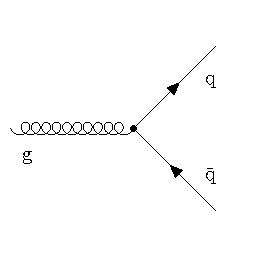
\includegraphics[width=0.33\textwidth]{figures/drawings/feynman/gqq.pdf}\hfill
    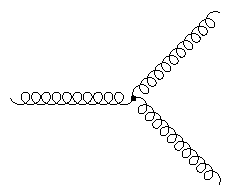
\includegraphics[width=0.33\textwidth]{figures/drawings/feynman/ggg.pdf}\hfill
    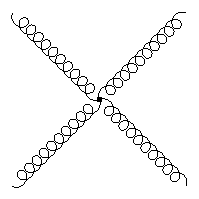
\includegraphics[width=0.33\textwidth]{figures/drawings/feynman/gggg.pdf}\hfill
    \caption[Fundamental vertices of QCD]{The fundamental Feynman rules of QCD
    comprise a quark-antiquark-gluon vertex, a three-gluon vertex and a 4-gluon
    vertex. The first two are proportional to $g_{s}$, the last one
    proportional to $g_{s}^2$.} 
    \label{fig:fundamental_couplings} 
\end{figure}

Unlike the other forces, the strong force force exhibits two unique and opposing
features. It is shown in experiments that quarks and gluons behave like free
particles at high energies or small distances, called \emph{Asymptotic freedom}
described in QCD by the falling of the strong coupling at high energies.
However, quarks and gluons cannot be observed as free particles at larger
distances. The strong force rise with increasing distance and the creation of
new quark-antiquark pairs are favored at some point. This phenomenon, called
\emph{confinement}, implies that the strong coupling increases at small energies
and is divergent. Consequently, perturbative QCD is not applicable in this
energy regime.

\subsection{Perturbative QCD}

All observables $X$ in perturbative QCD (pQCD) are developed as a
perturbative series in powers of the strong coupling \as. 

\begin{equation*}
    X = \sum_{n=0}^N \as^n c_i 
\end{equation*}

where $c_i$ are the perturbative coefficients. The expansion already yields
sufficiently accurate results after the first orders of the perturbative series,
if $\as \ll 1$ and the series converges quickly. However several features
complicate the perturbative calculations. Ultra-violet (UV) divergences enter
the calculations beyond leading order in form of loop corrections. The
divergences can be removed by a procedure called renormalization, see
Sec.~\ref{sec:renormalization}.

Soft and collinear divergences also need to be handled in perturbative
calculations. They arise from singularities at phase-space boundaries and
neglected quark masses. Observables need to be defined infrared safe and
short-distance effects need to be separated from the divergent long-range part,
which can be factorized into the PDFs, see Sec.~\ref{sec:factorization}.

\subsection{Renormalization and Running of the Strong Coupling}
\label{sec:renormalization}

Beyond LO, the calculations include loop corrections, which result in UV
divergences when calculating the momenta integrals of the loops. To make the
result finite, a regularization procedure called renormalization is applied. The
renormalization introduces another scale $\mur$, the renormalization scale.
There are different renormalization schemes, of which the
$\overline{\mathrm{MS}}$-scheme~\cite{Weinberg:1951ss,tHooft:1973mm} is the most
popular. Consequently the observable $X$ and the \as become functions of this
scale \mur. 

Nonetheless, the observable $X$ may not depend on the arbitrarily chosen \mur.
The renormalization group equation (RGE) states that the dependence of $X$ on
\mur must cancel. This can be mathematically expressed by

\begin{equation} 
    \mur^2 \frac{d}{d \mur^2} X \left(\frac{Q^2}{\mur^2},\as(\mur^2)\right) = \left(
    \mur^2 \frac{\partial X}{\partial \mur^2} + \mur^2 \frac{\partial
    \as(\mu^2)}{\partial \mur^2} \frac{\partial X}{\partial \as(\mu^2)} \right) \stackrel{!}{=} 0 
\end{equation}

and states that any dependence of $X$ on \mur must be cancelled by the
\mur-depedence of \as. Subsequently the strong coupling has to fulfill the
equation

\begin{equation}
    \mur^2 \frac{d \as}{d \mur^2} = \beta(\as) = - \left( \beta_0 \as^2 + \beta_1 \as^3
    + \beta_2 \as^4 + \ldots \right)
    \label{eq:as_rge}
\end{equation}

where $\beta_0$, $\beta_1$ and $\beta 2$ are the 1-loop, 2-loop and 3-loop 
$\beta$-function coefficients, which are given for the coupling of an effective
theory, in which the $n_f$ quark flavors are light ($m_q \ll \mur$). Here, they
are given in the $\overline{\mathrm{MS}}$-scheme.

\begin{equation} 
    \beta_0 = \frac{33 - 2 n_f}{12\pi}
\end{equation}

\begin{equation} 
    \beta_1 = \frac{153 - 19 n_f}{24\pi^2}
\end{equation}

\begin{equation} 
   \beta_2 = \frac{2857 -\left(\sfrac{5033}{9}\right)n_f + \left(\sfrac{335}{27}
   \right)n_f^2}{128 \pi^3}
\end{equation}

By integrating Eq.~\ref{as:rge} the energy dependence of \as is given. In an
enery range of constant number of flavors, an exact analytic solution exists in
1-loop approximation. 

\begin{equation*}
   \as(\mur^2) = \frac{1}{\beta_0 \ln \left( \sfrac{\mur^2}{\Lambda^2} \right)}
\end{equation*}

$\Lambda$ is the constant of the integration and corresponds to the scale at
which the perturbative coupling would diverege. Very often it is convenient to
give the strong coupling at a specific scale, from which the coupling at any
scale is calculated. It is common practice to report \asmz, consequently the
1-loop analytical function becomes

\begin{equation*}
   \as\left(\mur, \as(\mz)\right) = \frac{\as(\mz)}{1 + \as(\mz)\beta_0 \ln
       \left( \sfrac{\mur^2}{\mz^2} \right)}
\end{equation*}

\begin{figure}[htb] 
    \centering
    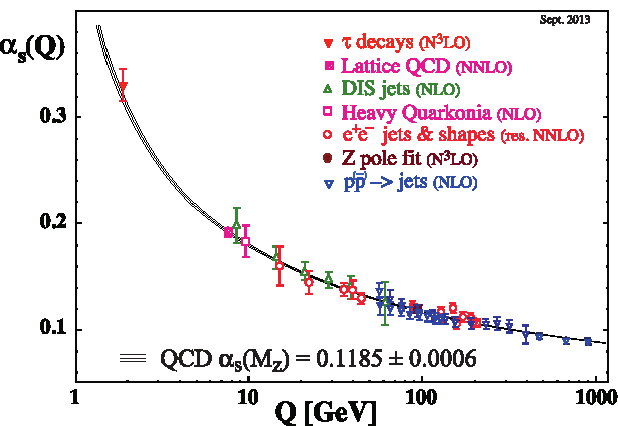
\includegraphics[width=0.95\textwidth]{figures/sm_model/as_running.pdf}\hfill
    \caption[Running of the strong coupling]{Running of the strong coupling
        constant as predicted by QCD. Determinations of the strong coupling from
        several experiments are shown at the scale of the measurement and prove
        the running up to \SI{1}{\TeV}. Recent measurements from
        CMS~\cite{Khachatryan:2014waa,CMS:2014mna} probe the running at even
        higher scales. Figure taken from~\cite{Agashe:2014kda}.} 
    \label{fig:as_running} 
\end{figure}


As the parameter is a free parameter of the theory, it is determined from
experimental measurements and evolved to the sclae of the $Z$-boson. The current
world average value of the strong coupling according to the
PDG~\cite{Agashe:2014kda} reads

\begin{equation*}
    \asmz = 0.1185 \pm 0.0006.
\end{equation*}

and is determined from hadronic $\tau$-lepton decaus, lattice QCD calculations,
deep-inelastic scattering data, electron-positron annihilation processes and
electroweak precision fits. Fig.~\ref{fig:as_running} shows various
determinations of the strong coupling constant from measurements at scales $Q$,
which describe the running of the strong coupling up to the \SI{1}{\TeV} scale.

\subsection{Factorization and Parton Density Functions}
\label{sec:factorization}

The perturbative series is only converging sufficiently fast for $\as(\mur) \ll
1$. As this is not given for low energies, perturbative calculations are not
applicable in this energy regime. 


The \emph{factorization theorem} separates the short-distance interactions,
which are calculated in the hard matrix element, from long-distance interactions
at an additionally introduced factorization scale \muf. This non-perturbative
long-distance part of the interaction is included in the parton distributions of
the proton. Consequently they PDFs cannot be calculated in pQCD, but have to be
determined experimentally.

\paragraph{DGLAP Evolution Equations}

Emissions which modify the momentum of a parton are to a large extent collinear
to the parton. The \emph{factorization theorem} describes the separation of
these long-distance interations from the short-distance interactions, the hard
process. The factorization again involes an arbitrary choice of factorization
scale \muf. Emission with transverse momenta above \muf are included in the hard
scattering perturbative coefficiencts while emission softer than \muf are
accounted for within the PDFs.

Consequently, the PDF depend on the scale \muf. The resulting dependence can be
described by the Dokshitzer-Gribov-Lipatov-Altarelli-Parisi (DGLAP) equations,
which are in LO defined as

\begin{equation*}
    \muf^2 \frac{\partial f_a (x, \muf^2)}{\partial \muf^2} = \sum_b \frac{\as(\muf^2)}{2 \pi} \int_x^1
    \frac{d z}{z} P_{ab}(z) f_b(\frac{x}{z}, \muf^2)
\end{equation*}

where $f_a$ is the parton distribution function of flavor $a$ and $P_{ab}$ are
the Altarelli-Parisi kernels, known as splitting functions. 

\paragraph{Parton Distribution Functions}

The structure of the proton is described by parton distribution functions
(PDFs). They represent the probability density\footnote{More precise a number
density as the PDFs are normalized to the number of partons.} to find a parton
carrying a momentum fraction $x$ of the proton momentum at a squared energy
scale $Q^2$. 

The DGLAP equations describe the evolution of the PDFs from a starting scale
$Q_0$ to an arbitray scale $Q$. However, the $x$-dependence of the PDFs as well
as the PDFs themselves at the starting scale $Q_0$ cannot be calculated, but
have to be derived from fits to data from experiments.

Several groups determine the proton PDFs in global fits to a large variety of
measurements from different experiments. Instead of determining all the 13
quark, antiquark and gluon PDFs independently, the number can be reduced by
choosing a sufficiently low starting scale $Q_0$ below the threshold of the
charm quark mass and calculating the heavy flavour PDFs in a heavy flavour
scheme~\cite{Thorne:2006qt}. Furthermore the PDF of the top and anti-top quark is
often neglected due to its large rest-mass. In the fits, each parton is
parametrized with sufficiently flexible function to the describe the $x$
dependence at the starting scale $Q_0$. The PDFs are evolved to the higher
scales of each measurement and the PDF parameters are adapted in an iterative
$\chisq$ fit.

Global PDFs are determined by the
CTEQ~\cite{Dulat:2015mca},MMHT~\cite{Harland-Lang:2014zoa},
NNPDF~\cite{Ball:2014uwa} and the ABM~\cite{Alekhin:2013nda} groups at LO, NLO
and NNLO. While the measurements which are put into the fit are often similar,
there are differences in the applied minimization method, phenomenological
approaches and the estimation of the uncertainties. More details are given in
Sec.~\ref{sec:pdf_uncertainties} in which the uncertainy of the PDFs on the
cross section measurement is discussed.

\begin{figure}[htb] 
    \centering
    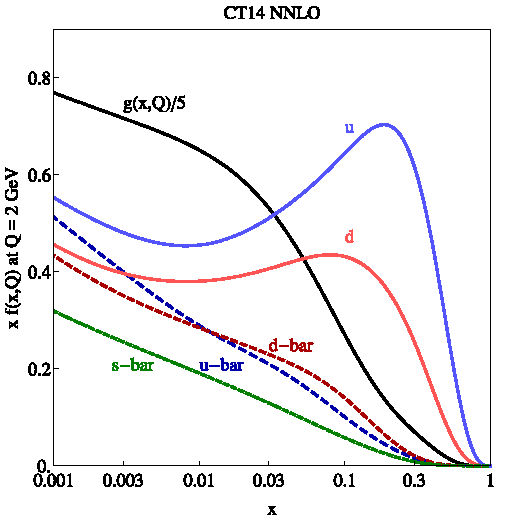
\includegraphics[width=0.49\textwidth]{figures/sm_model/ct14_2.pdf}\hfill
    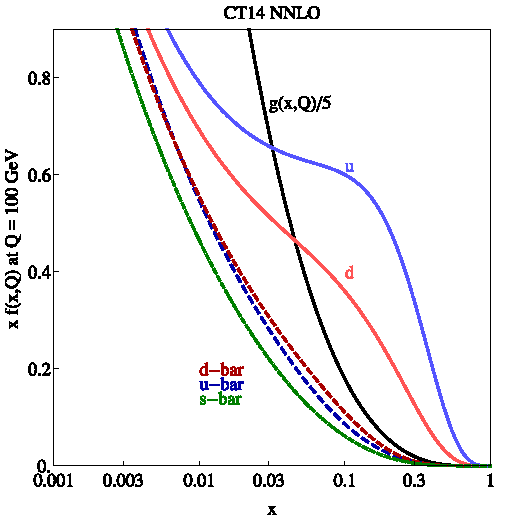
\includegraphics[width=0.49\textwidth]{figures/sm_model/ct14_100.pdf}
    \caption[CT14 NNLO PDF sets]{The CT14 NNLO PDF set with the gluon and quark
        PDFs at scale $Q=\SI{2}{\GeV}$ (left) and evolved to $Q=\SI{100}{\GeV}$
    (right) using the DGLAP evolution equations. Figure taken
    from~\cite{Dulat:2015mca}.}
    \label{fig:ct14_parton_distributions} 
\end{figure}

The HERAPDF group~\cite{Abramowicz:2015mha} uses a slightly different approach
by using a less flexible parameterization but restricting the data to
measurements from the HERA experiments, which provide a very precise and
compatible dataset. Furthermore the HERAPDF group released their fitting
framework HERAFitter~\cite{Alekhin:2014irh} as open source software, which can
be used by anyone.  HERAFitter is employed in Sec.~\ref{sec:pdf_constraints} to
study the constraints of the triple differential dijet measurements on the PDFs.

\begin{figure}[htb] 
    \centering
    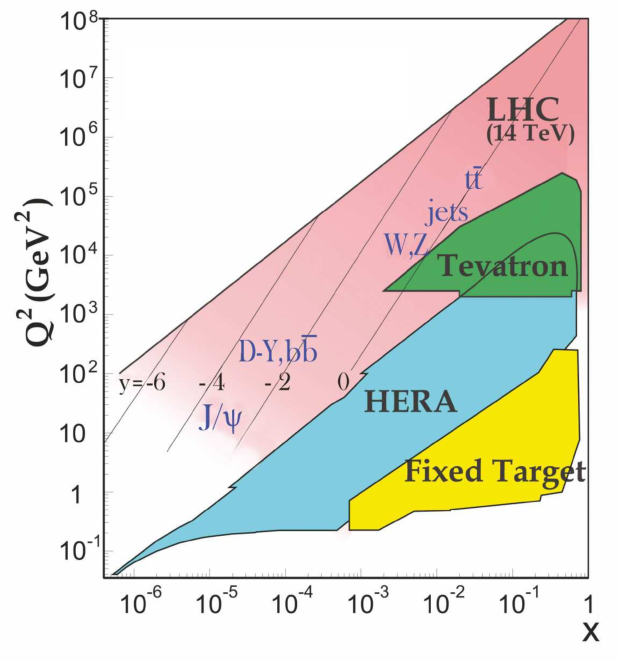
\includegraphics[width=0.8\textwidth]{figures/sm_model/phasespace.pdf}\hfill
    \caption[Kinematic phase space region of the experiments]{The phase space
        coverage in $x$ and $Q^2$ which is accessible in current experiments.
        The most important input for the PDFs still results from DIS data
        measured at HERA. Further important constraints at high $x$ and low
        scales are given by fixed-target experiments. The latest PDF sets also
        include LHC measurements with provide constraints at high scales $Q^2$
        and high-$x$ (jets, $t\bar t$) and at medium-$x$ ($W$,$Z$,+jets). Figure
        taken from~\cite{Agashe:2014kda}.} 
    \label{fig:kinematic_phasepace} 
\end{figure}

\section{Hadronization and Parton Shower}

As perturbative QCD calculations lack the capabilities of describing the
soft component of the interaction, additional models are employed which describe
the emission of additional partons and the hadronization into color-less bound
states. 

\subsection{Parton showers}

The accelerated colored partons undergo subsequent emission of gluons. Unlike in
QED radiation, gluons themselves carry color charge and therefore also emit
further gluons, leading to the parton shower. 

The dominant contributions come from collinear parton splitting and soft gluon
emissions. The collinear splitting of a parton is described by splitting
functions which are identical to the DGLAP splitting functions. The
subsequential application of the splitting to the colored particles leads to the
parton shower. The evolution of the shower is determined by an evolution
variable, \eg the virtual-mass squared of the partons in the shower. The upper
limit on the initial virtuality is given by the momentum transfer scale of the
hard process while the shower is terminated when the virtualities fall below the
hadronization scale, which is of the order of $\SI{1}{\GeV}$.

Actually the parton shower mimics the effect of effect of higher-order
corrections. As they are often not feasible to be calculated, the parton shower
approximation is instead used. Though great take has to be taken to avoid any
double counting if using a NLO generator in combination with a parton shower.

\subsection{Hadronization}

The result of the parton shower is a large number of color charged particles. As
color charged particles cannot be observed, they have to hadronize into bound
states which are color-less. The MC event generators Pythia and Herwig employ
different models to simulate the hadronization process. Pythia uses the Lund
string fragmentation model while Herwig is based on the cluster fragmentation
model.

\paragraph{Lund String Fragmentation Model}

Within the Lund string model, the attraction between a $q\bar q$ pair is
modeled through string, whose energy follows a coulomb potential as a function
of the distance between the two quarks. Final-state gluons from the parton
shower are considered as kinks in the strings. If the string exceeds a certain
threshold, it breaks up and new quark-antiquark pairs are formed. If the
available energy is too small, the quarks and antiquarks recombine into mesons
and baryons.

\paragraph{Cluster Fragmentation Model}

At first, all gluons are split into quark antiquark pairs. Neighbouring pais are
grouped together to form color-less clusters. Most of the clusters decay into
hadrons in an isotropic two-body phase space model.

\section{Jet Algorithms}
\label{sec:jet_algorithms}

The information of the clustered stream of particles, also known as jets,
provides the link between the short-scale physics and the final-state
observations. There are many different algorithms available which cluster jets
from a set of input objects. Both \CMS and \ATLAS rely on the \antikt and
inclusive-\kt jet algorithms, which proved to be very robust and both are
collinear and infrared safe, see Section~\ref{sec:coll_safety}. They are
sequential recombination algorithms and combine the input objects based on a
distance measure in Minkowski space. All jets were reconstructed using the
efficient algorithms implemented in the FastJet library~\cite{Cacciari:2011ma}.

\subsection{Collinear and Infrared Safety}
\label{sec:coll_safety}

Hard partons undergo many collinear splittings in the fragmentation process.
Additionally, there are always emissions of soft particles in QCD-like events
caused by non-perturbative and perturbative effects. The reconstructed jets
should be insensitive to all these effects. Furthermore, fixed-order pQCD
calculations are associated with divergent tree-level matrix elements and the
corresponding loop level matrix elements. While these divergences cancel for
infrared safe and collinear safe jet algorithms, this is not guaranteed for jet
algorithms not fulfilling the infrared and collinear safety requirements.
Fig.~\ref{fig:infrared_safety} shows the effect of a collinear splitting (right
plot) and of additional soft particles (left plot) on the results of an unsafe
jet algorithm. Most of the cone-based jet algorithms which cluster elements
by employing a constant distance measure in the $\eta-\phi$ space are affected by the
previously mentioned issues. This leads to the popularity of the modern sequential
recombination algorithms which are used in almost all of todays jet-based
analyses.

\begin{figure}[htb]
    \centering
    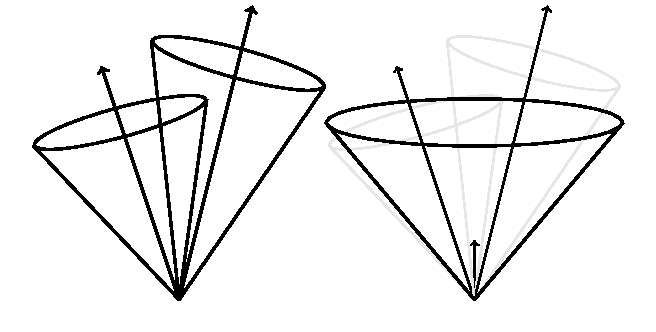
\includegraphics[width=0.45\textwidth]{figures/drawings/infrared_safety/jetinfrared.pdf}\hfill
    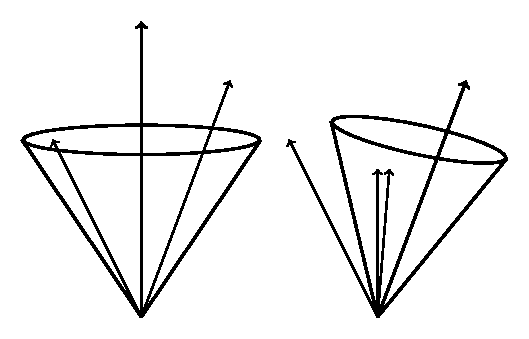
\includegraphics[width=0.45\textwidth]{figures/drawings/infrared_safety/jetcollinear.pdf}
    \caption[Effect of infrared emissions and collinear splittings on jet
    algorithms]{The influence of an infrared emission and a quasi
        collinear splitting on a jet algorithm not fulfilling the infrared safe
        and collinear safe requirements is shown. An additional soft particle (left plot)
    leads to the combination of the two jets into one large jet. A
quasi-collinear splitting of a particle (right plot) changes the result of the
jet clustering algorithm.}
    \label{fig:infrared_safety}
\end{figure}

\subsection{Generalized \kt Jet Algorithm}

The most popular sequential recombination algorithms are the \kt jet
algorithms which cluster jets based on a jet size parameter $R$ and an
additional parameter $p$, introducing a dependence on the transverse momentum of
the input objects. The pair-wise algorithm uses a list of input objects like stable
particles or particle flow candidates. 

At first, the distance $d_{ij}$ between two particles and the distances of the
particles to the beam $d_{iB}$ and $d_{jB}$ are calculated based on the rapidity
difference $\Delta y_{ij}$ and the azimuthal angle $\Delta \phi_{ij}$ between two
particles $i$ and $j$

\begin{align*} 
    d_{ij} &= \min(p_{\mathrm{T}i}^{2p},p_{\mathrm{T}j}^{2p})\frac{\left(\Delta
        R_{ij}\right)^2}{R^2}\\
    d_{i\mathrm{B}} &= k_{\mathrm{T}i}^{2p}
\end{align*} 

with the angular distance

\begin{align*}
    \left(\Delta R_{ij}\right)^2 &= (\Delta y_{ij})^2 + (\Delta \phi_{ij})^2
\end{align*} 

If distance $d_{ij}$ is smaller than the distances to the beam line, the two
particles $i$ and $j$ are merged into a new particle $k$ which then replaces the
particles $i$ and $j$ in the input list. These steps are repeated until all
particles are clustered into jets. Since the distance measures are defined in
Minkowski space, the shapes of the jets in the $\eta-\phi$ plane are not circular but
irregular, see Figure~\ref{fig:jet_shapes}. Based on the parameter $p$, there
are three important \kt based algorithms with distinct properties

\begin{figure}[htb]
    \centering
    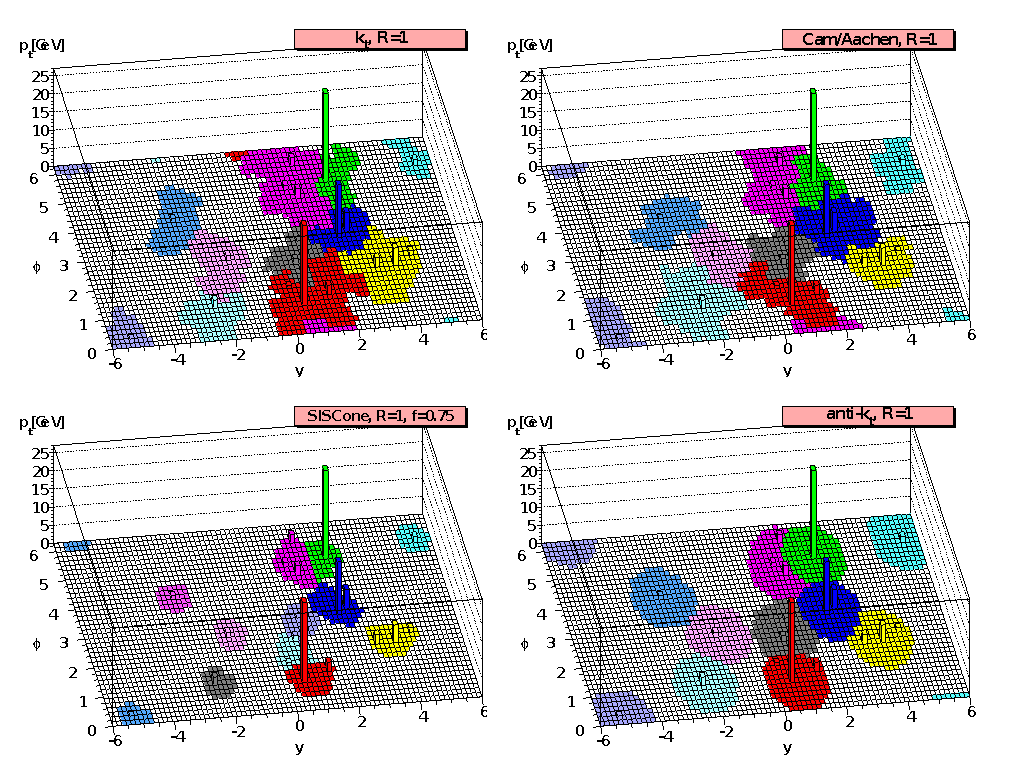
\includegraphics[width=0.8\textwidth]{figures/jet_reconstruction/jet_shapes.pdf}
    \caption[Jet areas of various jet algorithms]{Catchment areas of jets obtained by the described \kt-based algorithm
        and the cone-based SISCone algorithm~\cite{Salam:2009jx}. For most jet
        algorithms the shape is irregular, while the \antikt algorithm yields
        circular shapes for hard jets while soft jets are crescent shaped. Taken
        from~\cite{Berger:2014aca}.}
    \label{fig:jet_shapes}
\end{figure}

\begin{itemize}
    \item $p=1$: The \textbf{Inclusive $\mathbf{\kt}$
    algorithm}~\cite{Catani:1991hj,Catani:1992rm} is based on a \ptsq
        distance measure and approximately describes the inversion
        of the QCD branching process.
    \item $p=0$: The \textbf{Cambridge-Aachen
        algorithm}~\cite{Dokshitzer:1997in} is only based on the
        spatial separation of the objects and does not rely on the energy of
        the input objects. Similarly to the inclusive \kt algorithm its jets
        have an irregular shape. This jet algorithm is particularly interesting
        for jet substructure studies.
    \item  $p=-1$: The \textbf{anti-$\mathbf{\kt}$ algorithm}~\cite{Cacciari:2008gp} favours clustering hard input
        objects resulting in fairly circular jet shapes for hard jets, while
        soft jets are crescent-shaped if they are close to a hard jet.
\end{itemize}

\section{Dijet Production at Hadron-Hadron Colliders}

When two hadrons collide, the actual interaction takes place between the
constituents of the proton, the partons. Applying factorization, the total cross
sectiono of such a hard scattering of two hadrons $H_1$ and $H_2$ into a final
state $X$ can be expressed as

\begin{equation*}
    \begin{split}
    \sigma{H_1 H_2 \rightarrow X} = &\sum_{i,j} \int dx_1 dx_2 f_{i, H_1}
    \left(x_1, \muf^2 \right) f_{j,H_2} \left(x_2, \muf^2 \right) \\ 
    &\times \hat
    \sigma{i,j \rightarrow X} \left( x_1 P_1, x_2P_2, \as(\mur^2),
    \frac{Q^2}{\muf^2} \right)
\end{split}
\end{equation*}

where the sum runs over all contributing initial-state partons $i$ and $j$.
$f_{i}$ and $f_{j}$ denote the non-perturbative PDFs and $\hat \sigma $ the
perturbative hard scattering cross section.

\begin{figure}[htbp]
    \centering
    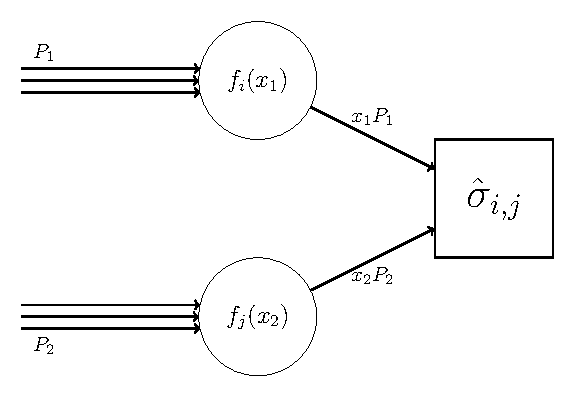
\includegraphics[width=0.5\textwidth]{figures/drawings/hardscattering.pdf}
    \caption[Factorization of hard scattering cross section.]
        {The total cross section is factorized into the hard scattering cross
        section and the PDFs.}
    \label{fig:dijet_cm_lab_frame}
\end{figure}
\todo{finalize figure}

\subsection{Kinematics of the Dijet System}

The outgoing partons of a hard interaction manifest themselves as a spray of
collimated particles, which are clustered into jets. Consequently, the
properties of jets are studied in order to gain a deeper understanding about
QCD and the proton structure. In the following disscussion, the partons
involved in the scattering process are assumed to be massless and collinear to
the beam protons. Furthermore, it is convenient to describe the kinematic of
the dijet system using the transverse momentum \pt and the rapidity $y$, as it
is introduced in Sec.~\ref{sec:coord_system}. 

The rapidity $y$, defined as

\begin{equation*}
    y = \frac{1}{2} \ln \left( \frac{E+p_z}{E-p_z} \right) 
\end{equation*}

is at lowest order directly related to the proton momentum fractions $x_1$ and
$x_2$ via

\begin{equation*}
    x_1 = \frac{x_\mathrm{T}}{2} \left( e^{y_1} + e^{y_2} \right)
    \qquad\text{and}\qquad x_2 = \frac{x_\mathrm{T}}{2} \left( e^{-y_1} +
    e^{-y_2} \right)
\end{equation*}
with $x_{\mathrm{T}} = \sfrac{\pt}{E}$ and the rapidities $y_1$ and $y_2$ of the
two outgoing partons.


\begin{figure}[htbp]
    \centering
    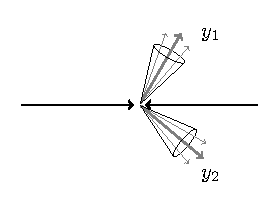
\includegraphics[width=0.45\textwidth]{figures/drawings/dijet_lab.pdf}
    \includegraphics[width=0.45\textwidth]{figures/drawings/dijet_cm.pdf}
    \caption[Dijet event in laboratory and center-of-mass frame.]
        {Dijet event in the laboratory frame (left) with the rapidities $y_1$
        and $y_2$ of the jets and in the center-of-mass frame (right) with the
    rapidities $\pm\ystar$.}
    \label{fig:dijet_cm_lab_frame}
\end{figure}

The longitudinal boost of the parton-parton center-of-mass (CM) frame with
respect to the proton-proton CM frame, \yboost, is calculated from the
rapidities $y_1$ and $y_2$ of the two jets emerging from the partons. 

\begin{equation*}
    \yboost = \frac{1}{2} |y_1 + y_2|
\end{equation*}

The quantities $\pm\ystar$ are the jet rapidities of the two jets in the
parton-parton CM frame. Since they are symmetric, \ystar is defined as half the
absolute rapidity separation between the two jets.

\begin{equation*}
    \ystar = \frac{1}{2} |y_1 - y_2|
\end{equation*}

\ystar is related to the polar scattering angle $\theta^*$ with respect to the
beamline by 

\begin{equation*}
    \ystar = \frac{1}{2} \ln \left( \frac{1 + |\cos \theta^*|}{1- | \cos \theta^*|} \right).
\end{equation*}
